\documentclass[12pt]{article}
\usepackage[a4paper, margin = 2cm]{geometry}
\usepackage[parfill]{parskip}    	
\usepackage{graphicx,caption,fancyhdr,xcolor,pdfpages,setspace, chronosys, lscape}
\usepackage{minted}
\usepackage{xcolor}

\usepackage[english]{babel}
\usepackage[square,numbers]{natbib}
\bibliographystyle{abbrvnat}

\usepackage[
        colorlinks = true,
        allcolors  = darkgray
]{hyperref}

\usepackage{tikz}
\usepackage{pgfgantt}
\usetikzlibrary{arrows,shapes,positioning,shadows,trees}
\usepackage[scale=1.0]{newtxtext,newtxmath}

\newcommand{\wrt}[1]{\mathrm{d}#1}

\setlength{\fboxsep}{0.5em}



\urlstyle{same}
\renewcommand{\footnoterule} % Push footnotes to the bottom of the page
	{\vfill\kern -3pt \hrule width 0.4\columnwidth \kern 2.6pt}

\makeatletter
\title{Design Construction \& Test for Audio}
\let\Title\@title
\author{Adam Gottesman}
\let\Author\@author
\date{Summer Term, 2023}
\let\Date\@date
\makeatother


\fancypagestyle{content}{
    \renewcommand{\headrulewidth}{0.4pt}
    \renewcommand{\footrulewidth}{0.4pt}
    \setlength{\headheight}{15pt}
    
	\fancyhf{}
	\fancyhead[L]{\Author}
	\fancyhead[R]{\Title}
	\fancyfoot[L]{\Date}
	\fancyfoot[R]{\thepage}
}


\begin{document}
\begin{titlepage}
\centering


\vspace{3cm}

{\LARGE \textbf{ Design, Construction \& Test for Audio}}



\vspace{2cm}

{\LARGE \textbf{ The School of Physics, Engineering and Technology}}

\vspace{2cm}
{\large \textbf{02/05/2023}}

\vspace{2cm}

{\LARGE \textbf{M2 Group Members:}}

{\large Ed Stubbs}

{\large Cian Downes}

{\large Tom Morrison}

{\large Jabez Cheung}

{\large \textbf{Adam Gottesman}}

{\large Duncan Sokolowski}







\vfill

{\itshape University of York}
\end{titlepage}

\tableofcontents
\newpage

\pagestyle{content}
\linespread{1}
\section{Introduction}


This report will document the path \texttt{Zen Sonic} has taken to design \texttt{Chaozzz}, an electronic musical instrument that shall meet the specification for this assessment. Firstly, the report will cover the entrepreneurial, technical, and environmental perspectives \texttt{Zen Sonic} has adopted since January 2023. Subsequently, a report of the individual contribution of the author will also be provided in addition to a reflective summary of \texttt{Zen Sonic}'s heretofore overall performance. 
\section{Entrepreneurial Report}
\subsection{Vision}
\texttt{Chaozzz} is the fruit of a collective attempt by \texttt{Zen Sonic} to transform \texttt{Hordijk}, a software synthesiser designed by the author in \texttt{Pure Data}, into a physically-controlled digital musical instrument. Although \texttt{Hordijk} is capable of making a wide range of interesting sounds, it is missing the tactile quality most hardware synthesisers possess as well as the ability to work without third-party software. By adapting \texttt{Hordijk} into \texttt{Chaozzz}, it will be possible for the target user, to explore deep sonic soundscapes and evolving rhythmic patterns, without a computer and certainly without any technical prerequisites. The aim of this product, therefore, is to enable our target user, to produce unique sounds and patterns without having to think too much about the way these sounds are made. Thus, \texttt{Chaozzz} aims to serve as a therapeutic rather than a strictly utilitarian instrument, which according to \texttt{Zen Sonic}, may significantly contribute to the well-being of the target user. 
\subsection{Target User}
Since the early 1990's, it has been proven through brain imaging and brain-wave analysis that music ``has a distinct influence on the brain by stimulating physiologically complex cognitive, affective, and sensorimotor processes" and thus it can be utilised ``to retrain and re-educate the injured brain"\cite{Neuro}.  This scientific confirmation of the power of music has led \texttt{Zen Sonic} to conclude that a musical instrument that can be played by anyone, without the need for any technical prerequisites, at the right price-point, may be precisely what needs to be designed in order to improve the mental health of as many people as possible. Considering the global increase in cases of emotional distress in capitalistic societies since the 1980's \cite{Sedated}, the ease of access to music production tools through digital technology, and the innate nature of the creative spirit of the human mind, it is possible to identify potential target users who could benefit from playing such an instrument. In \autoref{fig:venn}, it is clearly delineated that \texttt{Zen Sonic}'s target user lies at the intersection of a musician (in the sense of someone who derives pleasure from playing or composing music or manipulating sounds), a creative (in the sense of someone who derives pleasure from any form of creative activity), and someone experiencing some emotional distress, such as anxiety or depression.
\begin{figure}[ht]
    \centering
    \fbox{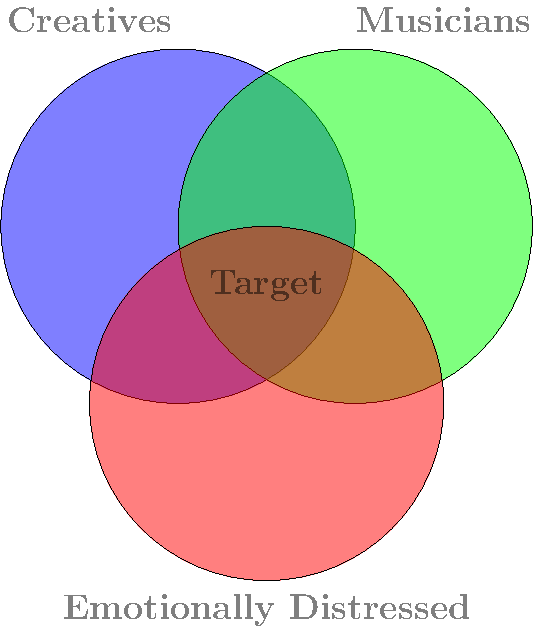
\includegraphics[width=0.25
    \textwidth]{Venn_Diagrams.pdf}}
    \caption{\texttt{Zen Sonic}'s target user.}%
    \label{fig:venn}
\end{figure}
\subsection{Marketing Strategies}
Now that \texttt{Zen Sonic}'s target user has been identified, the next necessary strategic step would be to think of ways to expose them to \texttt{Chaozzz}. \texttt{Zen Sonic} shall attempt to collaborate with various influencers from a variety of social media-platforms (e.g., youtube, twitch) who happen to be passionate about both well-being and music, by providing them with a Minimum Viable Product (\texttt{MVP}). This is mainly because it is not certain that a one-to-one adaptation of \texttt{Hordijk} into \texttt{Chaozzz} is precisely what the target user needs. Instead, only the core functionality of \texttt{Hordijk} will be designed, so that no wasted time is spent on designing a feature that may not interest the target user. What's more, \texttt{Zen Sonic} will attentively listen to what the beta-testers of \texttt{Chaozzz} might feel is missing, especially with regards to its overall functionality and user interface. \texttt{Zen Sonic} will also make use of digital marketing (i.e., website, promotional video) that will include testimonials that prove that \texttt{Chaozzz} has helped out users with their everyday life. Furthermore, \texttt{Zen Sonic} will continually attempt to partner up with trendy well-being brands such as Lululemon and SoulCycle, in order to expand into more product markets via trusted brands. The combination of constructive feedback from the beta-testers, the resultant word of mouth from social media platforms, as well as having the seal of approval from trusted brands, will enable \texttt{Zen Sonic} to positively expose \texttt{Chaozzz} to as many target users as possible while incrementally improving it throughout future versioning. 

\subsection{Additional Research}
In addition to developing the \texttt{MVP}, potential applications that \texttt{Chaozzz} could adopt over time will be explored. One of these applications include incorporating an alarm clock functionality within \texttt{Chaozzz}. Most alarm clocks are inherently dull and repetitive, while \texttt{Chaozzz} is meant to be a musical instrument that should consistently keep the target user entertained. By providing \texttt{Chaozzz} with the functionality to wake the target user up with interesting sounds and patterns, it could not only serve as a cure for anxiety or depression, but also as an aid to a healthy sleep cycle. The \texttt{Zen Sonic} team has already explored potential preset sounds for the alarm clock using the already built \texttt{Hordijk} software synthesiser in \texttt{Pure Data} during the development of the \texttt{MVP} (to listen, press \href{https://on.soundcloud.com/6Eg2s}{HERE}).

\subsection{Work Breakdown}
\subsubsection{Assessed Work}
In \autoref{fig:Gantt}, it can be clearly seen how \texttt{Zen Sonic} has planned to develop the prototype of the \texttt{MVP}. The main tasks are separated into three categories: Research \& Planning, Design \& Implementation, and Business \& Marketing. The green links illustrate the core steps that are required to successfully complete the prototype of the \texttt{MVP}, since one task, such as product testing, cannot be completed before the prototype is complete. Every other task that is required to meet the specification, with the exception of the video production, served as peripheral activities that could have been tackled at any point during the term.\footnote{We shall see later on in the Peer Assessment section that this was actually an inherent flaw in the work breakdown.} Provided in the appendix, a risk control timetable was designed by Duncan in order to ensure that \texttt{Zen Sonic} will not fall behind schedule. In practice, it ended up being completely unnecessary since this is a very small project and the scope of the assessment is for a relatively short duration. Yet it did give \texttt{Zen Sonic} confirmation that good progress was being made ahead of schedule. 
\begin{figure}[ht]
    \centering
    \fbox{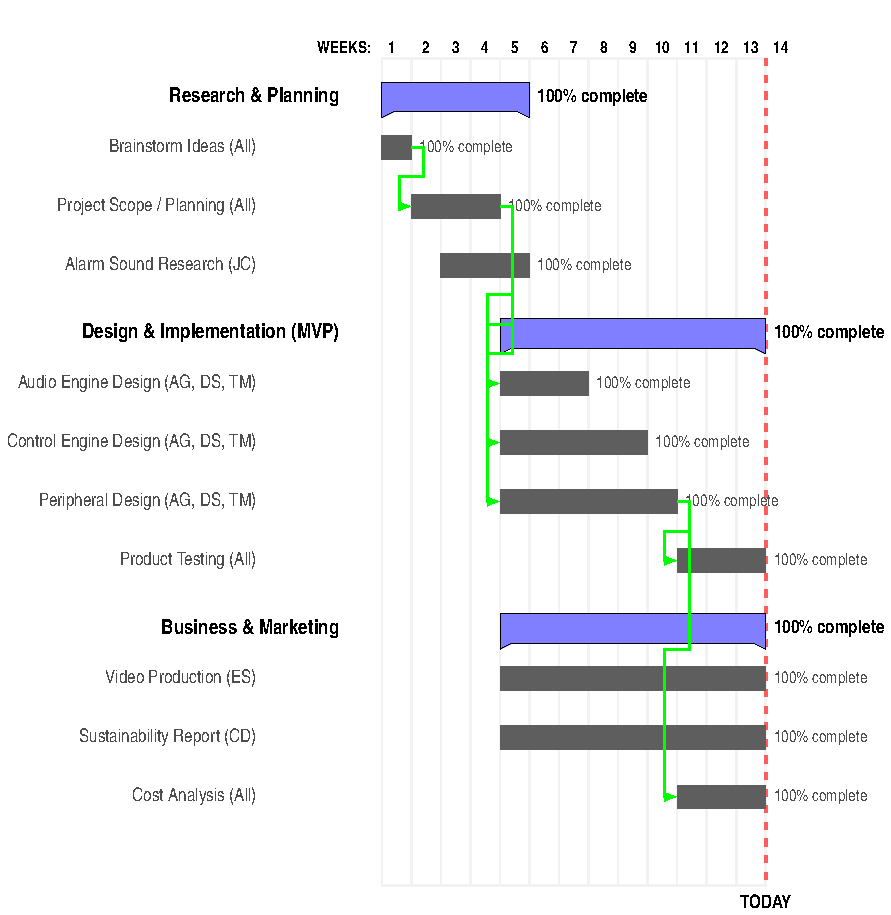
\includegraphics[width=0.7
    \textwidth]{Gantt.pdf}}
    \caption{Finalised Gantt Chart of the project.}
    \label{fig:Gantt}
\end{figure}

\subsubsection{Future Work}
\begin{figure}[ht]
    \centering
    \fbox{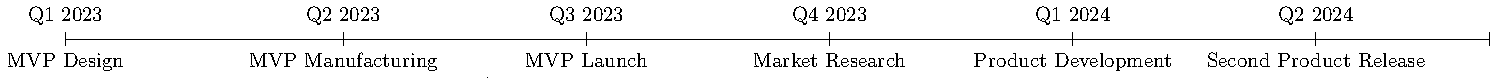
\includegraphics[width=0.9
    \textwidth]{roadmap.pdf}}
    \caption{Roadmap for the future of \texttt{Chaozzz}.}%
    \label{fig:roadmap}
\end{figure}

A work breakdown of the future of \texttt{Chaozzz} has also been constructed. The timeline in \autoref{fig:roadmap} indicates that:
\begin{itemize}
    \item Once the \texttt{MVP} prototype is complete in Q1 of 2023, \texttt{Zen Sonic} will focus on the manufacturing of the \texttt{MVP} in Q2 of 2023, such as the PCB and chassis design prior to the \texttt{MVP} launch in Q3 of 2023. 
    
    \item After the \texttt{MVP} will launch, market research will be conducted and feedback from the beta-testers will be collected during Q4 of 2023, so that design and manufacturing of the second product can commence by Q1 of 2024. 

    \item The second product will be released by Q2 of 2024 and by then, a new roadmap will be updated for the following year.
\end{itemize}

\section{Technical Report}
\subsection{Product Overview}
Instead of delving into the minute implementation details of \texttt{Chaozzz}, we will primarily focus on its structural underpinnings. The heart of \texttt{Chaozzz} is conceptually an amalgamation of two distinct engines: A \texttt{Control Engine} and an \texttt{Audio Engine}. 
\subsubsection{Control Engine}
It can be observed in \autoref{fig:control-engine}, that the \texttt{Control Engine} of the product consists of two oscillators, a \texttt{Data Oscillator} and a \texttt{Clock Oscillator}, being fed into the \texttt{Data Input} and \texttt{Clock Input} of a \texttt{Shift Register} respectively. It can be observed that there are two outputs that are tapped off the register, each comprising of a 4-bit binary value (since each cell can only store a \texttt{Logic High} or a \texttt{Logic Low}).\footnote{The \texttt{MVP} actually has 6-bit binary values per output. The fully-featured product would most likely incorporate three tapped outputs: one 4-bit binary value per oscillator and another 4-bit binary value for modulating a digital filter, which would process the sound coming out of the \texttt{FM Engine}: see \autoref{fig:audio-engine}.} Then, the binary value for each tapped output gets converted into a decimal value via a \texttt{Binary to Decimal Converter}, which is then fed back to its corresponding oscillator. It is also worth mentioning that the decimal value being fed back to its corresponding oscillator can be attenuated via a sensor so that the target user can have full control over the feedback configuration of the engine. One may ask, why would one design something of this sort? This type of design utilises a mechanism invented by Rob Hordijk called a \texttt{Rungler}, which simulates a dynamical system, since at first the parameters dictated by the target user instill certain initial conditions and over time, a pattern starts to stabilise as a consequence of these conditions\cite{Rungler}. This means that it will be able to generate chaotic musical patterns without the need of a keyboard or an onboard sequencer. It is also worth mentioning that the \texttt{MVP} has the added functionality of looping the chaotic pattern that had been generated with the use of a push-button. Now that we have a high level understanding of the \texttt{Control Engine}, we shall now cover the high level design of the \texttt{Audio Engine}.
\begin{figure}[ht]
    \centering
    \fbox{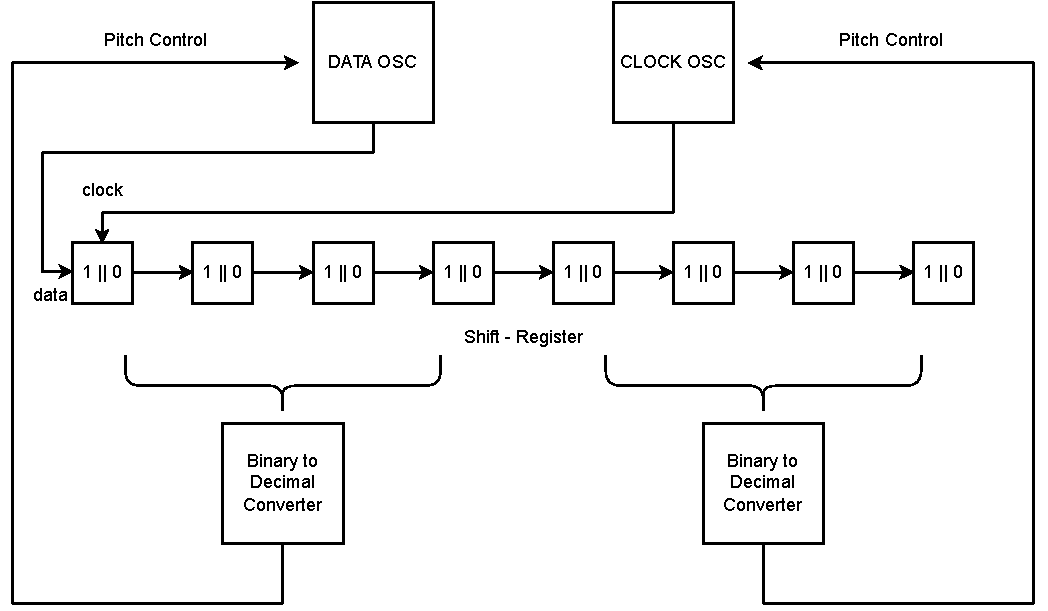
\includegraphics[width=0.6 \textwidth]{control_engine.pdf}}
    \caption{The Control Engine.}%
    \label{fig:control-engine}
\end{figure}
\subsubsection{Audio Engine}
It can be observed in \autoref{fig:audio-engine}, that the \texttt{Audio Engine} of the product consists of two oscillators, a \texttt{Data Oscillator} and a \texttt{Clock Oscillator}. These oscillators are both sinusoidal waveforms generated via standard wave-table synthesis techniques and they are both fed into an \texttt{FM Engine}. The \texttt{FM Engine} unsurprisingly offers frequency modulation synthesis capabilities, but it is designed in such a way that the \texttt{Data Oscillator} will serve as a carrier operand whereas the \texttt{Clock Oscillator} will serve as the modulator operand.\footnote{This is an intuitive way of looking at it but in practice, from an algorithmic perspective, the \texttt{Data Oscillator} and the \texttt{Clock Oscillator} are not strictly speaking operands of the \texttt{FM Engine} operator.} The frequency modulated signal in the current \texttt{MVP} will then be directly driven either with a loudspeaker or a headphone set (at the discretion of the target user). It is important to clarify that \texttt{Zen Sonic} decided to reserve the design of the filter and the \texttt{FX Engine} to future development as well as committing to keep the entire design of the synthesis engine within the digital domain. This would make the product much more affordable as well as ensure that preset capability could be implemented without potential digital / analogue interfacing issues during future versioning. Now that we have covered both the high-level design of the \texttt{Control Engine} and the \texttt{Audio Engine} of the \texttt{MVP}, we shall now assess whether \texttt{Zen Sonic} was able to design these engines within the provided specifications.
\begin{figure}[ht]
    \centering
    \fbox{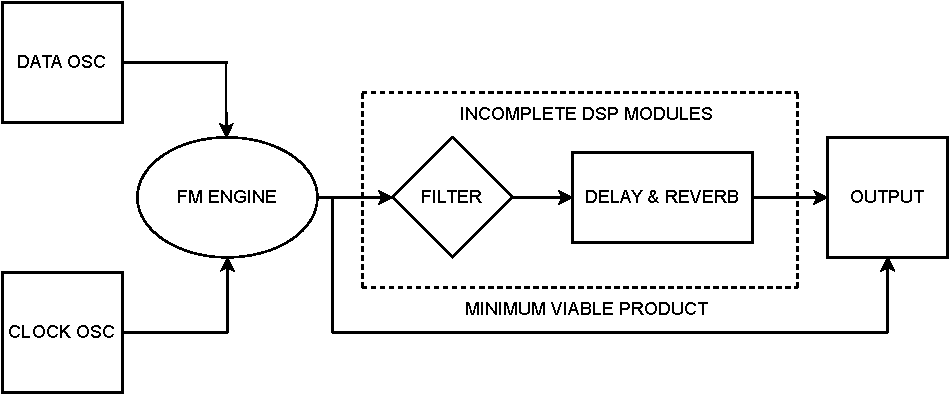
\includegraphics[width=0.6 \textwidth]{audio_engine.pdf}}
    \caption{The Audio Engine.}
    \label{fig:audio-engine}
\end{figure}
\subsubsection{Specification}
It can be confidently stated that \texttt{Zen Sonic} has managed to meet all of the specifications laid out prior to the submission date. The \texttt{MVP} operates and sounds the way it was intended to, the synthesis is completely based on code written for the \texttt{STM32F4}, and sensors, controlling the pitch of both the \texttt{Data Oscillator} and \texttt{Clock Oscillator}, the amount of frequency modulation in the \texttt{FM Engine}, and the amount of feedback sent back to both oscillators independently were successfully implemented well before the deadline. Even indicators displaying the logic state of every individual cell in the \texttt{Shift Register} have been implemented successfully. In fact, \texttt{Zen Sonic} has completed all of the technical requirements for the \texttt{MVP} prototype well in advance so that it would be possible to make a boastful demonstration of the product during the video production. It can be heard in the video production that the sound quality of the \texttt{MVP} is rich and that the user interface is intuitive. Henceforth, \texttt{Zen Sonic} is looking forward to further investigate various PCB and chassis designs so that the \texttt{MVP} will be manufactured with the same attention to detail as it was given to during its design.
\section{Sustainability Report}
Taking into account the sustainability factors of any product has become standard practice in industry. A recent article by the World Economic Forum states that "the message is loud and clear. Today, consumers around the world do want to live more sustainably"\cite{WEF}. They feel that "brands bear as much responsibility as governments". \texttt{Zen Sonic} has ensured to not deviate from these standard practices by considering how the carbon footprint and toxicity levels of the \texttt{MVP} can be minimised throughout its life-cycle. This approach has been taken by first considering the packaging, casing and circuitry of the \texttt{MVP} in order to adopt a coherent life cycle assessment (\texttt{LCA}).
\subsection{Packaging}
Many electronic devices require anti-static packaging in order to minimise the risk of it getting damaged from static charges during transportation. The sustainability team has advised that bags created out of wood pulp would be the most sustainably-friendly material for such purpose since they are much more disposable than polyethylene\cite{PULP}. There have been some disagreements regarding this strategy among the technical team since it would reduce the affordability of the \texttt{MVP}, but it was decided that since the manufacturing process will only commence in \texttt{Q2} of the product cycle, \texttt{Zen Sonic} will not dismiss this suggestion.  
\subsection{Casing}
The sustainability team has decided to use aluminium as the chassis material of the \texttt{MVP}. This is mainly because it is highly recyclable and its material quality remains intact throughout every recycling iteration. What's more, every time aluminium is recycled, only 5\% of the energy required to produce primary aluminium is exerted, making it also a low carbon footprint material\cite{ALUM}. The technical team is a bit concerned about the financial implications of such a decision but so far having aluminium as the casing material for the \texttt{MVP} is in line with \texttt{Zen Sonic}'s overall vision.
\subsection{Circuitry}
The sustainability team has suggested that the \texttt{PCB} substrate of the \texttt{MVP} should be biodegradable, since it would be made out of natural fibres unlike the generic glass-based fibre \texttt{PCB}s commonly used in industry. Furthermore, the sustainability team has also suggested to source the biodegradable \texttt{PCB} from Jiva Materials, since they claim that their \texttt{PCB}s' carbon footprint is 60\% lower than the typical \texttt{FR-4} \texttt{PCB}s \cite{JIVA}. The technical team, however, is a bit concerned that an alliance with such a specialised company is a bit far-fetched economically, and that certain compromises regarding sustainability are necessary in order to stay within the budget constraints of the \texttt{MVP}. Since the manufacturing process of the \texttt{MVP} will only take place during \texttt{Q2} of the product cycle, the suggestions from the sustainability team are still being kept into consideration. In addition to the \texttt{PCB}, \texttt{Zen Sonic} also has to take into consideration what active and passive components will be included in the \texttt{MVP} and where to source these materials from. 
\subsubsection{Active Components}
The core of the \texttt{MVP}'s functionality is undoubtedly embodied in the \texttt{STM32F4} microprocessor. Looking into STMicroelectronic's long term values, they place an active role in ensuring that they are sourcing materials responsibly and ethically for their products - as outlined in their long term values\cite{STM1}. They have enforced many requirements, such as ensuring that their suppliers conform to the \texttt{RMAP} standard, since  "they are screened to determine whether it falls under the scope of our Responsible Minerals Sourcing program"\cite{STM2}. Quoting their President of HR and CSR, she says that "[e]mbedding sustainability practices in our company strategy is essential to our people, our business, and society at large"\cite{STM3}. \texttt{Zen Sonic} can appreciate that they are making a huge commitment to ensure that they are sustainable, so in our product we can safely say that the \texttt{STM32F4} comes from a traceable and sustainable supply chain. Regarding the minerals used in the microprocessor, it is widely understood that some countries border on the line of violating human rights, and cause environmental damage. Looking through STMicroelectronic's policies and regulations, they are taking this very seriously. They understand that Tantalum, Tin, Tungsten and Gold are essential for their manufacturing processes, and therefore have a due diligence program in place to map their supply chains, so that the precious materials can be traced to their origins. Furthermore, they have assessments that require their smelters to take part in the Responsible Minerals Initiatives (\texttt{RMI}), so they can obtain validation that their metals are conflict-free; including being ethically sourced \cite{STM4}.

\subsubsection{Passive Components}
 According to the sustainability team, there are many economic benefits that can be oozed out of sourcing film resistors. Firstly, it is easier to recover e-waste from metal film resistors than from carbon film resistors, which means that they are more eco-friendly and economical\cite{MFresistor}. The sustainability team has also researched that metal knobs are usually chosen over plastic ones since they are easier to recycle \cite{RecoEwaste}. These observations from the sustainability team will ensure that \texttt{Zen Sonic} will be on the right path during the manufacturing stage of the \texttt{MVP}. 

\subsection{Life Cycle Assessment}

Throughout the design process of the \texttt{MVP}, \texttt{Zen Sonic} has constantly focused on the \texttt{LCA}. An \texttt{LCA} can be thought of as a company's total environmental impact. It goes from the initial stages of extracting those raw materials, all the way to manufacture, distribution and then disposal after the consumer uses the product. Below is a diagram, that suitably describes the process that happens:

\begin{figure}[h!]
    \centering
    \fbox{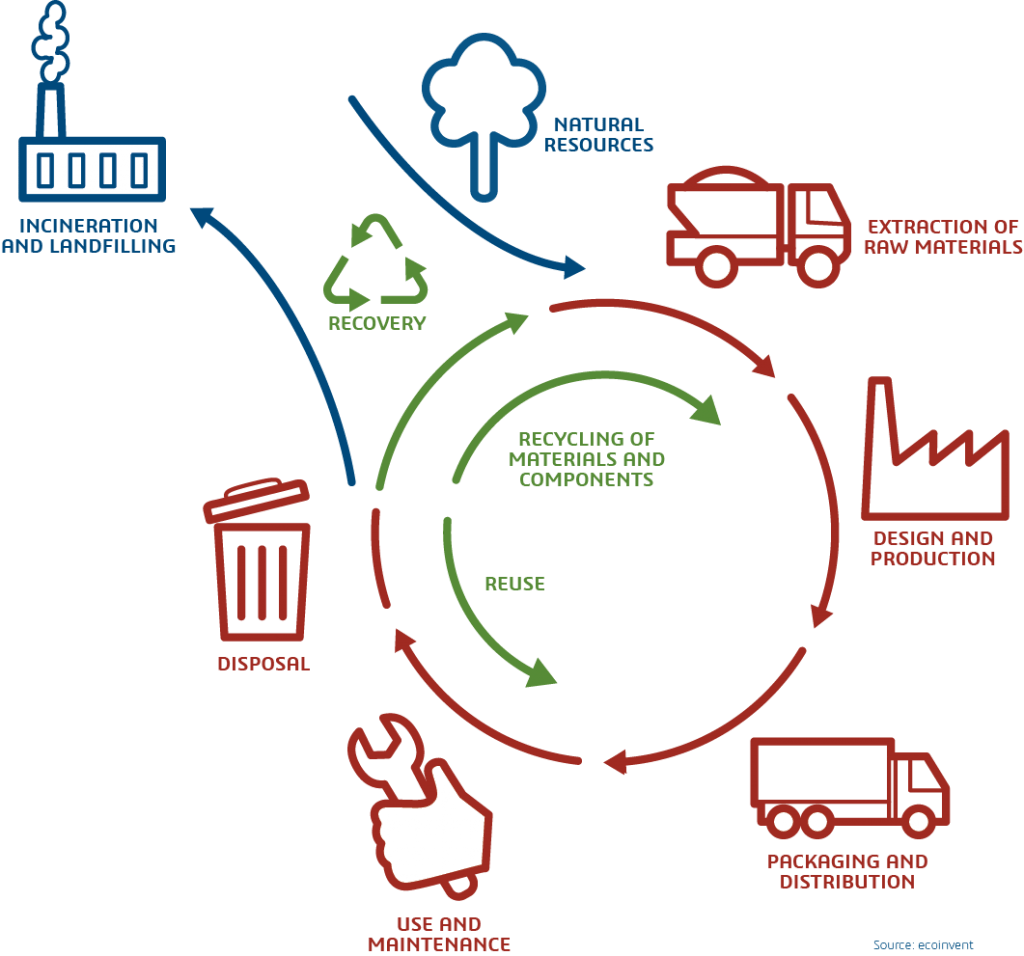
\includegraphics[width=0.3 \textwidth]{lca.png}}
    \caption{Life Cycle Assessment Diagram (taken from Dassault Systemes).}
    \label{fig:life-cycle}
\end{figure}

The designer plans to make the casing for the sequencer recyclable, along with the precious minerals on the PCBs. The aluminium casing waste during the manufacturing process could be recycled internally so that when new cases are being made, only the recycled material alongside the new one will be used. Aluminium extraction is intensive, and so recycling would also help the environment as less energy will be used in the process. The designer has also ensured that the sequencer is easily repairable by not using rare components, so that if a part of the \texttt{MVP} were to break, one would not need to replace the entire unit. This is not only beneficial for the target user, but also for the environment as it will not be necessary to extract more raw materials for the product. 


\section{Individual Contribution}
\subsection{List of Contributions}
\subsubsection{List of Everyone's Main Role}
\begin{itemize}
\item Ed Stubbs: In charge of Business and Marketing.
\item Tom Morrison: Embedded programming leader and head of software version control.
\item Duncan Sokolowski: In charge of record keeping and ensuring deadlines are met on time.
\item Cian Downes: Sustainability Leader.
\item Jabez Cheung: Schedules the weekly meetings and head of alarm clock research.
\item Adam Gottesman: Head of analogue engineering.
\end{itemize}



\subsubsection{List of the Author's Contributions}
\begin{enumerate}
\item Product Concept: The entire architecture of the \texttt{MVP} is based on the author's previous software synthesis project in \texttt{Pure Data}. In other words, both the \texttt{Control Engine} described in \autoref{fig:control-engine} and the \texttt{Audio Engine} in \autoref{fig:audio-engine} are entirely based on the author's original design and should count as a significant contribution to the project. Needless to say, these conceptual underpinnings accelerated \texttt{Zen Sonic}'s workflow since it significantly reduced the time required to meet the specification for this assessment.
\item Alarm Clock Research: The author has indirectly yet significantly contributed to the additional alarm clock research conducted by Jabez since it was the author's \texttt{Pure Data} synthesiser, which was used to create the presets.
\item Management: The author has created the Gantt chart in \autoref{fig:Gantt} and shared it with the rest of the team in order to convert Duncan's work breakdwon structure with a risk register (see Appendix) into a more human-readable work breakdown. 
\item \textbf{Analogue Engineering}: The author has been in charge of designing all of the peripheral circuitry as well as interfacing them with the \texttt{STM32F4 Discovery Board}. A detailed overview of the implementation details will be provided in the individual contribution section of the report.
\item Embedded Software Engineering: The author has significantly contributed to the software implementation and testing of the synthesis engine on the \texttt{STM32F4}. A detailed overview of the author's contribution, however, cannot be provided because it will result in exceeding the page limit for this report.  
\end{enumerate}




\subsection{Peripheral Hardware Design}
Even the most amazing processor in the world would be completely useless without a way of providing it data or outputting data from it. For this reason, both sensors and indicators were implemented in order to provide the \texttt{Control Engine} some data, and to display the real-time state of each cell in the \texttt{Shift Register} respectively.\footnote{Obviously, the most crucial peripheral in any electronic musical instrument is the speaker since it is the peripheral that converts electricity into acoustic energy, but since the driver for the audio output was not designed by \texttt{Zen Sonic}, and since the speaker that will be connected to the device is completely dependent on the target user's preferences, the author will not discuss the role of actuators and the implementation details of the audio driver that would drive them in the \texttt{MVP}.} We shall firstly cover the hardware implementation of the sensors and then proceed with a detailed overview of the hardware implementation of the indicators. 
\subsubsection{Sensors}
In order to transform the \texttt{MVP} into a tactile musical instrument, the use of potentiometers as sensors for controlling the instruments' various parameters had to be implemented by the author. At the current state of development of the synthesiser, multiple logarithmic 10k$\Omega$ potentiometers that single-handedly control the pitch of the \texttt{Clock Oscillator}, the pitch of the \texttt{Data Oscillator}, the depth of the \texttt{FM Engine}, and the chaotic feedback modulation amount for each oscillator were wired to their respective analogue input pins in the manner displayed in \autoref{fig:pot}. It can be clearly seen in \autoref{fig:pot} that the top terminal of each potentiometer is connected to the positive supply pin of the \texttt{STM32F4}, the middle terminal to its respective analogue pin, and the bottom terminal connected to common ground. This is a very conventional way of wiring a potentiometer in embedded systems, since the analogue pin will be able to read a range of voltage values predefined by the overall power supply range of the embedded device.

In practice:
\begin{itemize}
    \item The output pin of the potentiometer controlling the frequency of the \texttt{Data Oscillator} is connected to the pin representing \texttt{Pin 1} in \texttt{GPIO A}.
    
    \item The output pin of the potentiometer controlling the frequency of the \texttt{Clock Oscillator} is connected to the pin representing \texttt{Pin 2} in \texttt{GPIO A}.

    \item The output pin of the potentiometer controlling the modulation amount of the \texttt{FM Engine} is connected to the pin representing \texttt{Pin 3} in \texttt{GPIO A}.
    
    \item The output pin of the potentiometer controlling the amount of chaos modulation for the \texttt{Data Oscillator} is connected to the pin representing \texttt{Pin 6} in \texttt{GPIO A}.

     \item The output pin of the potentiometer controlling the amount of chaos modulation for the \texttt{Clock Oscillator} is connected to the pin representing \texttt{Pin 7} in \texttt{GPIO A}.
\end{itemize}

\begin{figure}[ht]
    \centering
    \fbox{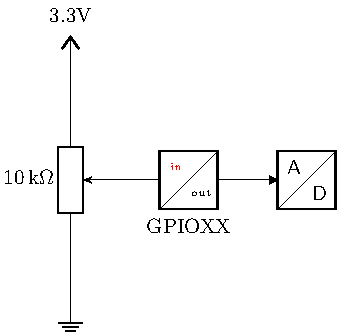
\includegraphics[width=0.25
    \textwidth]{pot.pdf}}
    \caption{Topology of the sensor configuration for the STM32F4.}
    \label{fig:pot}
\end{figure}

We have now covered all of the hardware implementation details pertaining to the sensors in the \texttt{MVP} and shall now move on to the hardware implementation details of the indicators. 

\subsubsection{Indicators}
In order to enhance the usability of the \texttt{MVP} as a therapeutic musical instrument, an \texttt{LED} display of the state of each cell within the \texttt{Shift Register} had been implemented by the author. Being able to receive visual feedback from the musical patterns generated in real-time, makes the experience of playing the instrument more intuitive and inspiring. It can be observed in \autoref{fig:led}, that a digital output of a pin representing pin X of GPIO X is connected to a current-limiting resistor, which is connected to an \texttt{LED}, which is connected to ground. This is a typical way of displaying the current state of a digital pin in an embedded system, but since each pin represents the logic state of a specific cell within the \texttt{Shift Register}, it is also possible to``see" the musical patterns generated by the \texttt{MVP}.
\begin{figure}[ht]
    \centering
    \fbox{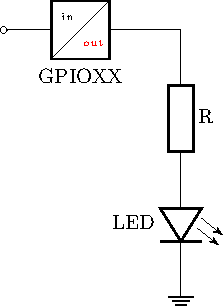
\includegraphics[width=0.2
    \textwidth]{led.pdf}}
    \caption{Topology of the LED display.}
    \label{fig:led}
\end{figure}
In practice:
\begin{itemize}
    \item Output pins \texttt{P0}, \texttt{P1}, \texttt{P2}, \texttt{P3} of \texttt{GPIO Port D} are each connected to their respective current limiting resistors, and each current limiting resistor is connected to its respective \texttt{Green LED}.

    \item Output pins \texttt{P5}, \texttt{P6}, \texttt{P7}, \texttt{P8} of \texttt{GPIO Port D} are each connected to their respective current limiting resistors, and each current limiting resistor is connected to its respective \texttt{Red LED}.

    \item Output pins \texttt{P0}, \texttt{P1}, \texttt{P2}, \texttt{P3} of \texttt{GPIO Port E} are each connected to their respective current limiting resistors, and each current limiting resistor is connected to its respective \texttt{Yellow LED}.
\end{itemize}

Last but not least, the author had to take into consideration what would be the optimal resistance values and minimum power rating requirements for the current limiting resistors for each \texttt{LED} colour in order to maximise the longevity of both the \texttt{LED}s and the current limiting resistors respectively.   

The author has also researched what resistor values are appropriate for our chosen \texttt{LED} colours by finding out the typical voltage drops across and the average current that is expected to flow through them\cite{LED}:

\begin{itemize}

\item 2.2V is the expected voltage drop across and 20mA is the average current that is expected to flow through a Green \texttt{LED}.

\item 1.8V is the expected voltage drop across and 20mA is the average current that is expected to flow through a Red \texttt{LED}.

\item 2.1V is the expected voltage drop across and 20mA is the average current that is expected to flow through a Yellow \texttt{LED}.
\end{itemize}

By applying basic circuit analysis techniques, we can mathematically express the resistance value for each current-limiting resistor:

\begin{equation*}
    R_\text{LED} = \left(V_\text{PSU} - V_\text{LED}\right) \,/\, I_\text{LED}
\end{equation*} where:

\begin{itemize}
    \item $R_\mathrm{LED}$ is the resistance of the current-limiting resistor.
    \item $V_\mathrm{PSU}$ is the voltage of the power supply.
    \item $V_\mathrm{LED}$ is the voltage drop across the \texttt{LED}.
    \item $I_\mathrm{LED}$ is the current flowing through the \texttt{LED}.
\end{itemize}

By plugging in the values into the equation, the current-limiting resistor for the Red, Green, and Yellow \texttt{LED}s turn out to be 75$\Omega$, 56$\Omega$ and 60$\Omega$ respectively (using \texttt{E-24} resistor values). In the same vein, it was also calculated that the Red, Green and Yellow \texttt{LED}s should be able to tolerate at least 30mW, 22mW, and 24mW respectively. 

To confirm that the theory matched reality, voltage drop measurements of each \texttt{LED} colour type were taken:

\begin{itemize}
    \item The voltage drop across the Red \texttt{LED} is 1.86V.
    \item The voltage drop across the Green \texttt{LED} is 1.93V.
    \item The voltage drop across the Yellow \texttt{LED} is 1.92V.
\end{itemize}

These are all the details required to correctly and efficiently implement the hardware aspects of the \texttt{MVP}'s indicators.

\subsection{Peripheral Interfacing}
Since we are dealing with an embedded system, simply wiring suitable components to the appropriate pins in the embedded device will not satisfy the correct operating conditions. Each pin connected to any component will need to be configured accordingly in embedded programming. The author will therefore discuss how the interface between the \texttt{STM32F4} and the peripherals was implemented.
\subsubsection{Sensors}
The author has decided to configure the pins connected to the output of the potentiometers as analogue inputs and decided to use the \texttt{Scan Mode} of the \texttt{ADC}, because it uses the Direct Memory Access (\texttt{DMA}) feature of the \texttt{STM32F4} to sense the readings from all of the potentiometers without any chance that the recorded data of one potentiometer will be overwritten by another. The way this is achieved is that on the input side of the \texttt{ADC}, the data recorded from the sensors will be stored in a table by a sequencer. Then, the recorded values from the table will be converted by the \texttt{ADC} in an order defined by an internal scheduler. Then, on the output end of the \texttt{ADC}, the converted data will be sent to memory via the \texttt{DMA}.

The first step required for implementing this type of configuration is by first initialising and configuring the \texttt{ADC}:
\begin{minted}{c}
void ADC_Config(void){
    /* Enable ADC1 clock */
    __HAL_RCC_ADC1_CLK_ENABLE();
    /* Configure ADC */
    myADC_handle.Instance = ADC1;
    myADC_handle.Init.ClockPrescaler = ADC_CLOCK_SYNC_PCLK_DIV8;
    myADC_handle.Init.Resolution = ADC_RESOLUTION_8B;
    myADC_handle.Init.ScanConvMode = ENABLE;
    myADC_handle.Init.ContinuousConvMode = ENABLE;
    myADC_handle.Init.DiscontinuousConvMode = DISABLE;
    myADC_handle.Init.ExternalTrigConvEdge =  ADC_EXTERNALTRIGCONVEDGE_NONE;
    myADC_handle.Init.DataAlign = ADC_DATAALIGN_RIGHT;
    myADC_handle.Init.NbrOfConversion = 5;
    myADC_handle.Init.DMAContinuousRequests = ENABLE;
    myADC_handle.Init.EOCSelection = ADC_EOC_SEQ_CONV;
    HAL_ADC_Init(&myADC_handle);
}
\end{minted}
It can be seen that \texttt{ADC1} has been initialised, that \texttt{ScanConvMode} has been enabled, that the number of conversion has been set to 5 (since there are five potentiometers requiring conversions), and so forth. This is an example of how the \texttt{HAL} library abstracts away the complex bare-metal implementations required to configure the \texttt{ADC} to successfully convert data from multiple sensors simultaneously.

The next required step is to configure the \texttt{GPIO} pins to be set accordingly:
\begin{minted}{c}
void GPIO_Config(void){
    /* Peripheral clock enable (Port A) */
    __HAL_RCC_GPIOA_CLK_ENABLE();
    /* Initialise Pin1, Pin1, Pin2, Pin3, Pin6 and Pin7 
     * on port A as Analog */
    myAnalogGPIO.Pin  = GPIO_PIN_1 | GPIO_PIN_2 | GPIO_PIN_3 |
                        GPIO_PIN_6 | GPIO_PIN_7;
    myAnalogGPIO.Mode = GPIO_MODE_ANALOG;
    myAnalogGPIO.Pull = GPIO_NOPULL;
    HAL_GPIO_Init(GPIOA, &myAnalogGPIO);
}
\end{minted}
It can be seen that Pin 1, Pin 2, Pin 3, Pin 6, and Pin 7 of \texttt{GPIOA} have all been enabled and set to analogue mode in human-readable code thanks to the abstraction features of the \texttt{HAL} library.

The last step required is to configure the \texttt{DMA} itself:
\begin{minted}{c}
void DMA_Config(ADC_HandleTypeDef *hadc){
     /* DMA2 clock enable */
    __HAL_RCC_DMA2_CLK_ENABLE();
    /* Initialise DMA2 */
    myDMA2_handle.Instance = DMA2_Stream0;
    myDMA2_handle.Init.Channel = DMA_CHANNEL_0;
    myDMA2_handle.Init.Direction = DMA_PERIPH_TO_MEMORY;
    myDMA2_handle.Init.PeriphInc = DMA_PINC_DISABLE;
    myDMA2_handle.Init.MemInc = DMA_MINC_ENABLE;
    myDMA2_handle.Init.PeriphDataAlignment = DMA_PDATAALIGN_BYTE;
    myDMA2_handle.Init.MemDataAlignment = DMA_MDATAALIGN_BYTE;
    myDMA2_handle.Init.Mode = DMA_CIRCULAR;
    myDMA2_handle.Init.Priority = DMA_PRIORITY_LOW;
    myDMA2_handle.Init.FIFOMode = DMA_FIFOMODE_DISABLE;
    HAL_DMA_Init(&myDMA2_handle);
    /* Link DMA2 to ADC1 */
    __HAL_LINKDMA(hadc,DMA_Handle,myDMA2_handle);
}
\end{minted}
It can be seen that channel 0 of stream 0 of \texttt{DMA2} was selected to send the converted data from the \texttt{ADC} to memory and various initialisation parameters were used to configure it. The \texttt{DMA} is then linked to the \texttt{ADC} via an encapsulated linker function included in the \texttt{HAL} library. The author would like to emphasise that the code written for this part of the assignment is heavily adapted from a tutorial series on \texttt{youtube} covering how to correctly configure the \texttt{ADC} for multiple input readings\cite{MUTEX}. Since the sensors had been implemented in hardware and configured in software, it is now imperative to test whether it works. Below is an image confirming that multiple readings are being read by the \texttt{ADC}:
\begin{figure}[ht]
    \centering
    \fbox{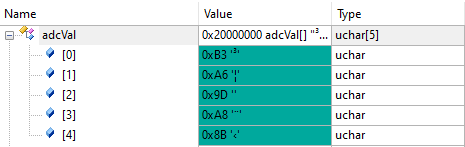
\includegraphics[width=0.75
    \textwidth]{sensor.png}}
    \caption{Test confirming multiple sensor readings.}
    \label{fig:sensor}
\end{figure}

\subsubsection{Indicators}
Interfacing the indicators with the microprocessor is much more straightforward than for the sensors. Firstly, the pins wired to the \texttt{LED}s must first be initialised:
\begin{minted}{c}
void LEDInit(void){
    /* Peripheral clock enable (Port D) */
    __HAL_RCC_GPIOD_CLK_ENABLE();
    /* Initialise Pins from port D */
    myDigitalGPIOD.Pin  = GPIO_PIN_0 | GPIO_PIN_1 | GPIO_PIN_2 |
                          GPIO_PIN_3 | GPIO_PIN_5 | GPIO_PIN_6 |
                          GPIO_PIN_7 | GPIO_PIN_8;			 
    myDigitalGPIOD.Mode = GPIO_MODE_OUTPUT_PP;
    myDigitalGPIOD.Pull = GPIO_PULLUP;
    HAL_GPIO_Init(GPIOD, &myDigitalGPIOD);
    /* Peripheral clock enable (Port E) */
    __HAL_RCC_GPIOE_CLK_ENABLE();	
    /* Initialise Pins from port E */
    myDigitalGPIOE.Pin  = GPIO_PIN_0 | GPIO_PIN_1 | GPIO_PIN_2 |
                          GPIO_PIN_3;			 
    myDigitalGPIOE.Mode = GPIO_MODE_OUTPUT_PP;
    myDigitalGPIOE.Pull = GPIO_PULLUP;
    HAL_GPIO_Init(GPIOE, &myDigitalGPIOE);
}
\end{minted}

It can be observed that all of the initialised pins are chosen as outputs, that they were all set to push/pull modes and pull up modes. The latter may seem nonsensical, but the pull up mode is chosen because it could prevent undefined behaviour if at some point the push/pull configuration will be switched to open drain. Then these abstracted parameters provided by the \texttt{HAL} library will initialise all of the required pins thanks to the \texttt{HAL\_GPIO\_Init} function. The last step required for the indicators to display the logic state of each cell in the \texttt{Shift Register} is by assigning these states to the \texttt{BSRR} of both \texttt{GPIOD} and \texttt{GPIOE} via simple bit shifting and masking operations. The operation where a logic 1 is assigned to every relevant register of the \texttt{BSRR} prior to assigning the \texttt{Shift Register} states is there to reset the display for each register since without it the \texttt{LED}s would end up blinking so quickly that it would be impossible to perceptually keep track of what is going on:   
\begin{minted}{c}
void updateDisplay(void){
    GPIOD -> BSRR  = ((1  <<  0) << 16) |
                     ((1  <<  1) << 16) |
                     ((1  <<  2) << 16) |
                     ((1  <<  3) << 16) |
                     ((1  <<  5) << 16) |
                     ((1  <<  6) << 16) |
                     ((1  <<  7) << 16) |
                     ((1  <<  8) << 16);
    GPIOD -> BSRR |= (shiftReg[0]   <<  0) |
                     (shiftReg[1]   <<  1) |
                     (shiftReg[2]   <<  2) |
                     (shiftReg[3]   <<  3) |
                     (shiftReg[4]   <<  5) |
                     (shiftReg[5]   <<  6) |
                     (shiftReg[6]   <<  7) |
                     (shiftReg[7]   <<  8);
    GPIOE -> BSRR  = ((1  <<  0) << 16) |
                     ((1  <<  1) << 16) |
                     ((1  <<  2) << 16) |
                     ((1  <<  3) << 16);			 
    GPIOE -> BSRR |= (shiftReg[8]   <<  0) |
                     (shiftReg[9]   <<  1) |
                     (shiftReg[10]  <<  2) |
                     (shiftReg[11]  <<  3);
\end{minted}
Since the indicators had been implemented in hardware and configured in software, it is now imperative to test whether it works. \autoref{fig:indicator} confirms that the \texttt{Shift Register} values are being updated during run-time. It is hard to prove that it works with a simple screenshot but a quick glance at the video production will make it clear that the \texttt{LED} display is working as intended.
\begin{figure}[ht]
    \centering
    \fbox{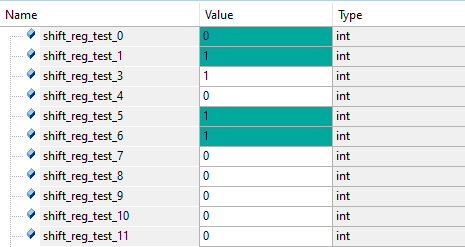
\includegraphics[width=0.4
    \textwidth]{indicator.png}}
    \caption{Test confirming that the indicator values are being updated.}
    \label{fig:indicator}
\end{figure}

\section{Peer Review}
\subsection{Overall Group Performance}
Overall, the group has performed very well. From the onset, concrete roles were assigned to each member and in most cases, each member has committed to what they were supposed to deliver. There has been, however, an intrinsic flaw in the prioritisation of our work breakdown (presented in the Entrepreneurial Report section). We have decided to make the technical side of the project heavily monitored while allowing a lot of freedom in terms of scheduling for less technical aspects of the project. This has resulted in a gamble. What ended up happening is that the marketing and business team has done an excellent job while the sustainability team has done a fairly poor job. This has occurred due to not having tighter measures to monitor the progress of every peripheral activity (from an engineering perspective at least). Retrospectively, it would have been better if the team spent more time on allocating suitable roles for certain members since it is clear that giving extra freedom to someone who we do not yet know we can trust can be a very risky strategy. All things considered, however, the gamble was not too bad since we have managed to meet the technical specifications for this assessment as well as provide a promotional video we are proud of.  

\subsection{Mark Allocation}
Ed Stubbs - Ed has decided from the onset that he would rather focus on the marketing, story-board for the video, as well as the video production itself instead of being part of the technical or research team. This decision has made our lives so much easier since the technical team had enough time to fulfill the required specifications without having to stress too much about producing the promotional video of the product. The group eventually ended up working on the video together, but Ed without a doubt was the mastermind behind that task. Mark: 20

Duncan Sokolowski - Duncan primarily undertook a managerial role and has partially contributed to the technical development of the product. It was great working with Duncan since he consistently ensured that everything was on schedule and was keen on understanding all of the technical intricacies of the embedded programming so he could contribute during the product development. Mark: 20 

Tom Morrison - Tom has primarily been delegated as the software leader of the team. In practice, however, he has not contributed to the technical development of the software as much as I had expected. This was primarily due to the fact that he has not spent any significant time beyond the allocated hours to work on the project, and as a result, it was not possible for him to make enough progress during the product development. He has, however, always been present throughout the entire process and has been very helpful during the allocated hours. Mark: 20

Jabez Cheung - Jabez was officially the manager of the team. It is true that he has ensured that group meetings were not missed and that enough progress has been made throughout the product development. He has also spent a significant amount of time on the alarm clock research, which has helped us think about the future potential of our product. These contributions, however, were not particularly vital for achieving the required specifications so it may be concluded that his contribution was fairly marginal. Mark: 5

Cian Downes - Cian was in charge of the environmental report of the project. His contribution has been fairly disappointing. Throughout the development of the product, he has been consistently late and at times absent. He has not contributed much overall although it did seem to be as a result of some personal struggles throughout the term. Also looking over the work that he did produce, it was of poor quality and seems to have discrepancies in the way in which it was produced. Mark: 0

Adam Gottesman- I was assigned to be the analogue engineer of the product. What happened in practice, however, was that I ended up leading the technical development of the product since week 4/5. This situation occurred because I felt that Duncan and Tom were not able to progress quickly enough in order to meet the specification for the MVP so I had to extend my allocated time as the analogue engineer and focus in addition on the embedded programming for the project. Eventually, I ended up designing a significant portion of the software and hardware of the project. Furthermore, although this is not technically a contribution, I also had to resort to researching about the sustainability aspects of the \texttt{STM32F4} and spending extra time thinking about the \texttt{LCA} because the sustainability team did not take it seriously enough. Mark: 35.
\newpage
\bibliography{bib}
\newpage
\section{Appendix}
\subsection{Duncan's Work Breakdown Structure with Risk Register}
\begin{figure}[ht]
    \centering
    \fbox{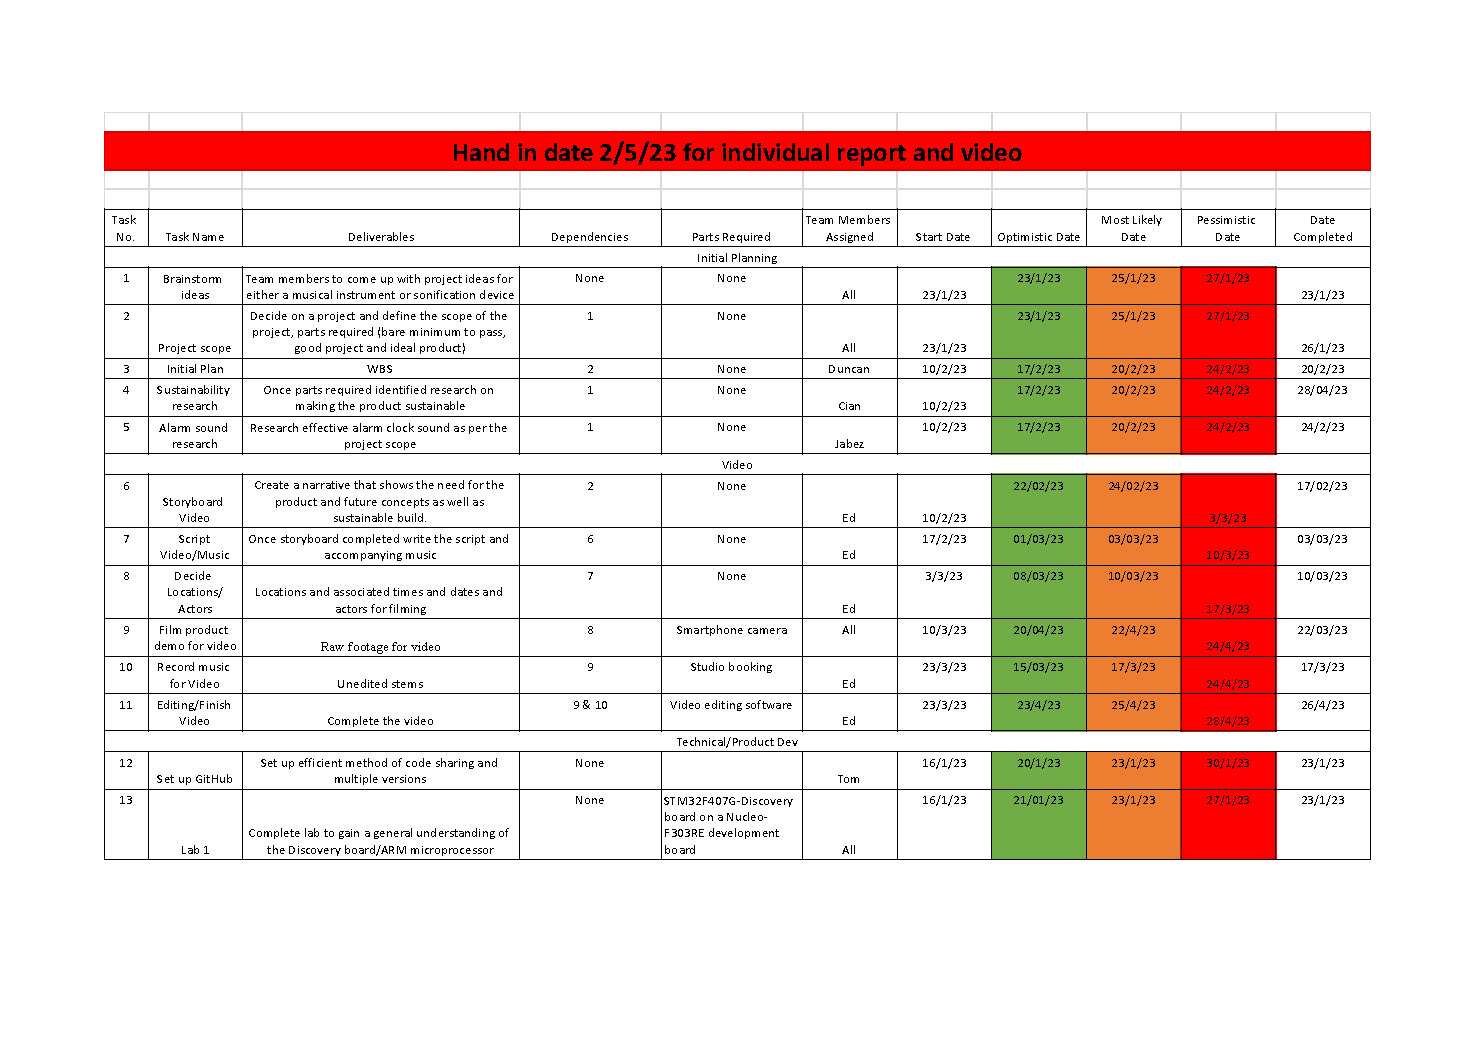
\includegraphics[width=0.9
    \textwidth]{WBS1.pdf}}
    \caption{Part I of Duncan's WBS with a risk register.}
    \label{fig:WBS1}
\end{figure}
\newpage
\begin{figure}[ht]
    \centering
    \fbox{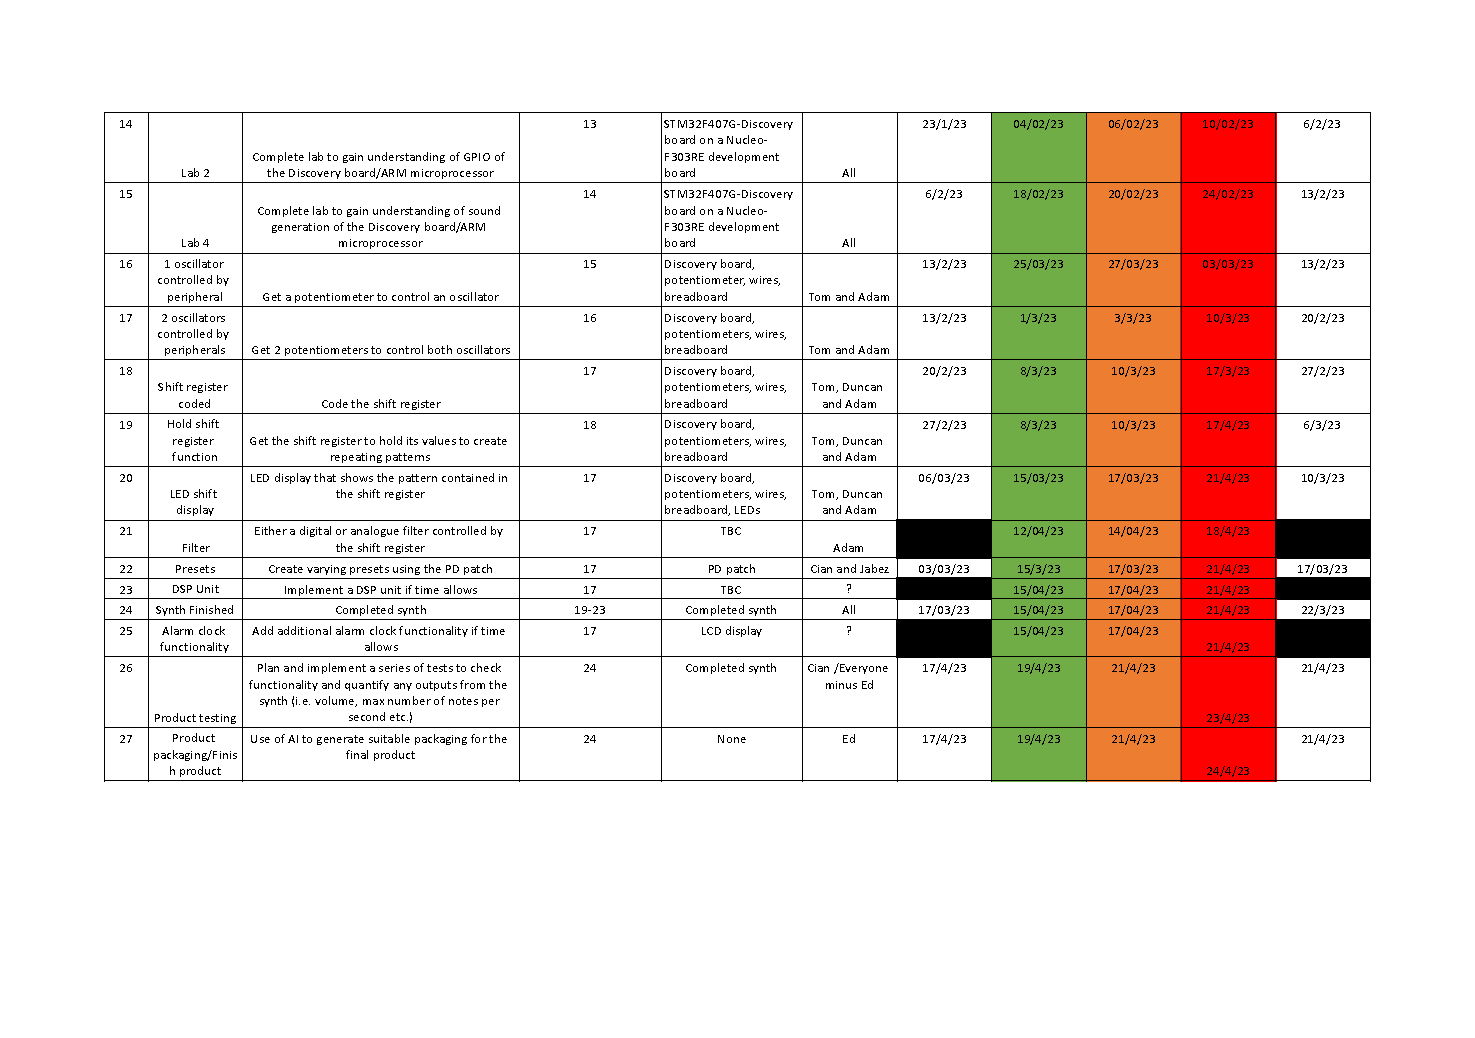
\includegraphics[width=0.9
    \textwidth]{WBS2.pdf}}
    \caption{Part II of Duncan's WBS with a risk register.}
    \label{fig:WBS2}
\end{figure}
\newpage


\subsection{Source Code}
\begin{minted}{c}

#include "./Drivers/Audio_Drivers.h"
#include "stm32f4xx_hal.h"
#include <stdlib.h>
#include <stdbool.h>
#include <math.h>

#define PBSIZE 4096
#define SINELOOKUPSIZE 16192
#define SINESIZE 16192
#define PI 3.141592653589793
#define REG_MAX 12

/* Functions prototypes -----------------------------------------------------*/
void GPIO_Config(void);
void DMA_Config(ADC_HandleTypeDef*);
void ADC_Config (void);
void myAudioHalfTransferCallback(void);
void myAudioTransferCompleteCallback(void);
void synthInit(void);
void buildOsc(int16_t*);
void emptyBuffer(int16_t*);
void checkBufferStatus(void);
void updateOscFreq(void);
void updateFreqMod(void);
void shift(void);
void streamAudio(int);
void binToDec(void);
void updateShiftReg(void);
void LEDInit(void);
void updateDisplay(void);
void holdInit(void);
/* --------------------------------------------------------------------------*/

/* Global variables ---------------------------------------------------------*/
uint8_t adcVal[5];

int16_t sineBuff_1[SINESIZE];
int16_t sineBuff_2[SINESIZE];
int16_t playBuff[PBSIZE];
int16_t currSample_2;
int16_t nextSample_1;
int16_t nextSample_2;
uint32_t startFill = 0;
uint32_t endFill = 0;
int hold = 0;

enum eNoteStatus {ready, going, finish} noteStatus = ready; 
enum eBufferStatus {empty, finished, firstHalfReq, firstHalfDone, 
    secondHalfReq, secondHalfDone} bufferStatus = empty;

DMA_HandleTypeDef myDMA2_handle;
ADC_HandleTypeDef myADC_handle;
ADC_ChannelConfTypeDef ADC_ChConfg;
GPIO_InitTypeDef myAnalogGPIO;
GPIO_InitTypeDef myDigitalGPIOD;
GPIO_InitTypeDef myDigitalGPIOE;

int shiftReg[12] = {0, 0, 0, 0,
                    0, 0, 0, 0,
		    0, 0, 0, 0};
										
float chaosMod_1;
float chaosMod_2;
																						
float f_1;
float f_2;

float currentPhase_1; 
float currentPhase_2;
	
float phaseInc_1; 
float phaseInc_2;

float modPhase_1;
float modPhase_2;

float modPhaseInc_1;
float modPhaseInc_2;

float modDepth;
float modAmount_1;
float modAmount_2;
/* --------------------------------------------------------------------------*/


/* MAIN PROGRAM -------------------------------------------------------------*/
int main(void) {

    /* ADC SETTINGS -----------------------------------------------------------*/
    GPIO_Config();
    DMA_Config(&myADC_handle);
    ADC_Config();
    HAL_ADC_Start_DMA(&myADC_handle, (uint32_t*)adcVal, 5);
    /* ------------------------------------------------------------------------*/
    
    /* BUFFER SETTINGS --------------------------------------------------------*/
    emptyBuffer (playBuff);
    myAudioSpeedUpTheSystemClock(); 
    initAudioTimer();     
    myAudioInitialisePeripherals(OUTPUT_DEVICE_AUTO, 80, AUDIO_FREQUENCY_44K); 
    myAudioStartPlaying(playBuff, PBSIZE);
    /* ------------------------------------------------------------------------*/
	
    /* SYNTH SETTINGS -------------------------------------------------------- */
    synthInit();
    buildOsc(sineBuff_1);
    buildOsc(sineBuff_2);
    /* ------------------------------------------------------------------------*/
	
    /* LED SETTINGS -----------------------------------------------------------*/
    LEDInit();
    /* ------------------------------------------------------------------------*/

    /* Initialise blue button -------------------------------------------------*/
    holdInit();
    /* RUNTIME OPERATION ----------------------------------------------------- */
    while(true) {
        checkBufferStatus(); 
        if (startFill != endFill) {
            for (int i = startFill; i < endFill; i += 2) {		
					
                updateOscFreq();
                updateFreqMod();
                updateShiftReg();
                updateDisplay();
                streamAudio(i);
            }
        }
    }
    /* ------------------------------------------------------------------------*/
}
/* --------------------------------------------------------------------------*/

/* ADC Functions ------------------------------------------------------------*/
void GPIO_Config(void){
	
    /* Peripheral clock enable (Port A) */
    __HAL_RCC_GPIOA_CLK_ENABLE();
	
    /* Initialise Pin0, Pin1, Pin2 on port A as Analog */
    myAnalogGPIO.Pin  = GPIO_PIN_1 | GPIO_PIN_2 | GPIO_PIN_3 |
                        GPIO_PIN_6 | GPIO_PIN_7;
    myAnalogGPIO.Mode = GPIO_MODE_ANALOG;
    myAnalogGPIO.Pull = GPIO_NOPULL;
    HAL_GPIO_Init(GPIOA, &myAnalogGPIO);
}
void DMA_Config(ADC_HandleTypeDef *hadc){
	
    __HAL_RCC_DMA2_CLK_ENABLE();
	
    myDMA2_handle.Instance = DMA2_Stream0;
    myDMA2_handle.Init.Channel = DMA_CHANNEL_0;
    myDMA2_handle.Init.Direction = DMA_PERIPH_TO_MEMORY;
    myDMA2_handle.Init.PeriphInc = DMA_PINC_DISABLE;
    myDMA2_handle.Init.MemInc = DMA_MINC_ENABLE;
    myDMA2_handle.Init.PeriphDataAlignment = DMA_PDATAALIGN_BYTE;
    myDMA2_handle.Init.MemDataAlignment = DMA_MDATAALIGN_BYTE;
    myDMA2_handle.Init.Mode = DMA_CIRCULAR;
    myDMA2_handle.Init.Priority = DMA_PRIORITY_LOW;
    myDMA2_handle.Init.FIFOMode = DMA_FIFOMODE_DISABLE;
    HAL_DMA_Init(&myDMA2_handle);
	
    /* Link this DMA to ADC1 */
    __HAL_LINKDMA(hadc,DMA_Handle,myDMA2_handle);
}

void ADC_Config(void){
	
    /* Enable ADC1 clock */
    __HAL_RCC_ADC1_CLK_ENABLE();
	
    /* Configure ADC */
    myADC_handle.Instance = ADC1;
    myADC_handle.Init.ClockPrescaler = ADC_CLOCK_SYNC_PCLK_DIV8;
    myADC_handle.Init.Resolution = ADC_RESOLUTION_8B;
    myADC_handle.Init.ScanConvMode = ENABLE;
    myADC_handle.Init.ContinuousConvMode = ENABLE;
    myADC_handle.Init.DiscontinuousConvMode = DISABLE;
    myADC_handle.Init.ExternalTrigConvEdge =  ADC_EXTERNALTRIGCONVEDGE_NONE;
    myADC_handle.Init.DataAlign = ADC_DATAALIGN_RIGHT;
    myADC_handle.Init.NbrOfConversion = 5;
    myADC_handle.Init.DMAContinuousRequests = ENABLE;
    myADC_handle.Init.EOCSelection = ADC_EOC_SEQ_CONV;
    HAL_ADC_Init(&myADC_handle);
	
    /* ADC Channel-1 */
    ADC_ChConfg.Channel = ADC_CHANNEL_1;
    ADC_ChConfg.Rank = 1;
    ADC_ChConfg.SamplingTime = ADC_SAMPLETIME_3CYCLES;
    HAL_ADC_ConfigChannel(&myADC_handle, &ADC_ChConfg);

    /* ADC Channel-2 */
    ADC_ChConfg.Channel = ADC_CHANNEL_2;
    ADC_ChConfg.Rank = 2;
    ADC_ChConfg.SamplingTime = ADC_SAMPLETIME_3CYCLES;
    HAL_ADC_ConfigChannel(&myADC_handle, &ADC_ChConfg);
	
    /* ADC Channel-3 */
    ADC_ChConfg.Channel = ADC_CHANNEL_3;
    ADC_ChConfg.Rank = 3;
    ADC_ChConfg.SamplingTime = ADC_SAMPLETIME_3CYCLES;
    HAL_ADC_ConfigChannel(&myADC_handle, &ADC_ChConfg);
    
    /* ADC Channel-4 */
    ADC_ChConfg.Channel = ADC_CHANNEL_6;
    ADC_ChConfg.Rank = 4;
    ADC_ChConfg.SamplingTime = ADC_SAMPLETIME_3CYCLES;
    HAL_ADC_ConfigChannel(&myADC_handle, &ADC_ChConfg);
    
    /* ADC Channel-5 */
    ADC_ChConfg.Channel = ADC_CHANNEL_7;
    ADC_ChConfg.Rank = 5;
    ADC_ChConfg.SamplingTime = ADC_SAMPLETIME_3CYCLES;
    HAL_ADC_ConfigChannel(&myADC_handle, &ADC_ChConfg);
}
/* --------------------------------------------------------------------------*/

/* Audio Buffer Functions -------------------------------------------------- */
void myAudioHalfTransferCallback(void){ 
    bufferStatus = firstHalfReq; 
} 
void myAudioTransferCompleteCallback(void) {    
    myAudioChangeBuffer(playBuff, PBSIZE);    
    bufferStatus = secondHalfReq; 
}
void emptyBuffer (int16_t *playBuff){
	
    for(int i = 0; i <= PBSIZE; i++) 
        playBuff[i] = 0;
}
void checkBufferStatus(void){
	
    startFill = 0;
    endFill = 0;
				
    if (bufferStatus == firstHalfReq){
        startFill = 0;
        endFill = PBSIZE / 2;
        bufferStatus = firstHalfDone;
    }
    else if (bufferStatus == secondHalfReq){
        startFill = PBSIZE / 2;
        endFill = PBSIZE;
        bufferStatus = secondHalfDone;
    }
}
void streamAudio(int i){	
	
    /* AUDIO OUTPUT */ 
    playBuff [i]     = nextSample_1;
    playBuff [i + 1] = nextSample_1;
}
/* --------------------------------------------------------------------------*/

/* LED Functions ------------------------------------------------------------*/
void LEDInit(void){
	
    /* Peripheral clock enable (Port D) */
    __HAL_RCC_GPIOD_CLK_ENABLE();
	
    /* Initialise Pins from port D */
    myDigitalGPIOD.Pin  = GPIO_PIN_0 | GPIO_PIN_1 | GPIO_PIN_2 |
                          GPIO_PIN_3 | GPIO_PIN_5 | GPIO_PIN_6 |
                          GPIO_PIN_7 | GPIO_PIN_8;
											 
    myDigitalGPIOD.Mode = GPIO_MODE_OUTPUT_PP;
    myDigitalGPIOD.Pull = GPIO_PULLUP;
    HAL_GPIO_Init(GPIOD, &myDigitalGPIOD);
	
    /* Peripheral clock enable (Port E) */
    __HAL_RCC_GPIOE_CLK_ENABLE();
	
    /* Initialise Pins from port D */
    myDigitalGPIOE.Pin  = GPIO_PIN_0 | GPIO_PIN_1 | GPIO_PIN_2 |
                          GPIO_PIN_3;
											 
    myDigitalGPIOE.Mode = GPIO_MODE_OUTPUT_PP;
    myDigitalGPIOE.Pull = GPIO_PULLUP;
    HAL_GPIO_Init(GPIOE, &myDigitalGPIOE);
}

void updateDisplay(void){
	
    GPIOD -> BSRR  = ((1  <<  0) << 16) |
                     ((1  <<  1) << 16) |
                     ((1  <<  2) << 16) |
                     ((1  <<  3) << 16) |
                     ((1  <<  5) << 16) |
                     ((1  <<  6) << 16) |
                     ((1  <<  7) << 16) |
                     ((1  <<  8) << 16);

 
    GPIOD -> BSRR |= (shiftReg[0]   <<  0) |
                     (shiftReg[1]   <<  1) |
                     (shiftReg[2]   <<  2) |
                     (shiftReg[3]   <<  3) |
                     (shiftReg[4]   <<  5) |
                     (shiftReg[5]   <<  6) |
                     (shiftReg[6]   <<  7) |
                     (shiftReg[7]   <<  8);
 	
    GPIOE -> BSRR  = ((1  <<  0) << 16) |
                     ((1  <<  1) << 16) |
                     ((1  <<  2) << 16) |
                     ((1  <<  3) << 16);
				 
    GPIOE -> BSRR |= (shiftReg[8]   <<  0) |
                     (shiftReg[9]   <<  1) |
                     (shiftReg[10]  <<  2) |
                     (shiftReg[11]  <<  3);			 
}
	
/* HOLD control -------------------------------------------------------------*/
void holdInit(void) {
	
    /* Set the blue button as an input */
    GPIOA->MODER &= ~GPIO_MODER_MODER0;
	
}

/* --------------------------------------------------------------------------*/
/* Audio synthesis Functions ------------------------------------------------*/
void buildOsc(int16_t *sineBuff){
	
    /* Set up the sine look-up table for osc1 */ 
    for (int i = 0; i < SINESIZE; i++) {
        float q = (32760 * sin(i * 2.0 * PI / SINESIZE)) * 0.25f;    
        sineBuff [i] = (int16_t) q; 
    }
}
void synthInit(void){
	
    modPhase_1 = 0.0f;
    modPhase_2 = 0.0f;

    modDepth = 0.5f;
    modAmount_1 = 0.5f;
    modAmount_2 = 0.5f;

    currentPhase_1 = 0.0f; 
    currentPhase_2 = 0.0f;
	
    f_1 = 220.0f; 
    f_2 = 440.0f;
	
    phaseInc_1 = (float)SINELOOKUPSIZE * f_1 / AUDIO_FREQUENCY_44K; 
    phaseInc_2 = (float)SINELOOKUPSIZE * f_2 / AUDIO_FREQUENCY_44K;
}

void updateOscFreq(void){
	
    currSample_2 = nextSample_2;
	
    /* Readings from ADC1 for OSC 1 ) */
    f_1 = ((adcVal[0] * 3.1f) * (1.0f + (1.0f * ((chaosMod_1 / 40.0f) * 
        (adcVal[3]  / 128.0f))))) + 25.0f;
				
    phaseInc_1 = SINELOOKUPSIZE * f_1 * (1.0f + modAmount_1) / 
        AUDIO_FREQUENCY_44K;
	
    currentPhase_1 += phaseInc_1;
				
    if ( currentPhase_1 > SINELOOKUPSIZE ) 
        currentPhase_1 -= SINELOOKUPSIZE ;
				
    nextSample_1 = sineBuff_1[( uint16_t )( currentPhase_1 )];
				
    /* Readings from ADC1 for OSC 2  */
    f_2 = ((adcVal[1] * 0.05f) * (1.0f + (1.0f * ((chaosMod_2 / 40.0f) * 
        (adcVal[4] / 128.0f)))));
				
    phaseInc_2 = SINELOOKUPSIZE * f_2 / AUDIO_FREQUENCY_44K;
	
    currentPhase_2 += phaseInc_2;
				
    if (currentPhase_2 > SINELOOKUPSIZE) 
        currentPhase_2 -= SINELOOKUPSIZE ;
				
    nextSample_2 = sineBuff_2 [(uint16_t)(currentPhase_2)];
}

void updateFreqMod(void){
	
    /* Osc 1 FM where readings of Osc 2 characterise the modulation */
    modPhaseInc_1 = (SINELOOKUPSIZE * f_2 * 20.0f / 
        (AUDIO_FREQUENCY_44K * 2.0f));
	
    modPhase_1 += modPhaseInc_1;	
				
    if (modPhase_1 > SINELOOKUPSIZE) 
        modPhase_1 -= SINELOOKUPSIZE;
										
    /* Readings from ADC1 for FM depth */
    modDepth    =  adcVal [ 2 ] / 64.0f;
    modAmount_1 = (modDepth * sineBuff_1[(uint16_t)modPhase_1] / 32768.0f);
}

void shift(void){

    int value;
    int newBit = shiftReg[REG_MAX - 1];
    if (nextSample_1 > 0)
        value = 1;
    else
        value = 0;
		
    for (int i = REG_MAX; i > 0; i--) 
        shiftReg[i] = shiftReg[i - 1];
	
    if ( GPIOA->IDR & GPIO_IDR_ID0 ) 
        shiftReg[0] = newBit;
    else 
        shiftReg[0] = value;
}

void binToDec(void){
	 
    chaosMod_1 =    (shiftReg[0] << 0) +
                    (shiftReg[1] << 1) +
                    (shiftReg[2] << 2) +
                    (shiftReg[3] << 3) +
                    (shiftReg[4] << 4) +
                    (shiftReg[5] << 5);
	
    chaosMod_2 = (shiftReg[6]   << 0) +
                 (shiftReg[7]   << 1) +
                 (shiftReg[8]   << 2) +
                 (shiftReg[9]   << 3) +
                 (shiftReg[10]  << 4) +
                 (shiftReg[11]  << 5);
}

void updateShiftReg (void) {
	
    if (currSample_2 < 0 && nextSample_2 > 0){ 
        shift();
        binToDec();	
    }
}
/* --------------------------------------------------------------------------*/
\end{minted}
\newpage


\end{document}  

